\section{\textit{Hierarchical Clustering}}
\subsection{Pengertian \textit{Hierarchical Clustering}}
\hspace{1cm}Strategi pengelompokan hierarchical clustering umumnya ada dua jenis yaitu Agglomerative (Bottm-Up) dan Devisve (Top-Down). Algoritma agglomerative hierarchical clustering dikarenakan; hasil dari pengelompokan data dapat dilihat dendrogram, tidak diperlukan penentuan jumlah cluster pada awal pengelompokan, dan agglomerative hierarchical clustering dengan pendekatan bawah-atas (buttom-up) dimana pengelompokan data dimulai dari kecil ke pengelompokan yang besar. 
\par\hspace{0.5cm}Agglomerative hierarchical clustering (AHC) dengan menggunakan buttom-up, dimulai dari masing-masing data sebagai sebuah cluster, kemudian secara rekrusif mencar kelompok terdekat sebagai pasangan yang kemudian akan digabungkan menjadi kelompok yang lebih besar. Proses tersebut diulang terus sehingga tampak bergerak keatas membentuk hirarki .
\par\hspace{1cm}Terdapat tiga teknik kedekatan dalam hierarchical clustering, yaitu; single linkage (jarak terdekat) atau tautan tunggal, average linkage (jarak rata-rata) atau tautan rata-rata,dan complete linkage (jarak terjauh) atau tautan lengkap.\citep*{pujakusuma2017pengelompokan}.

\subsection{Langkah-langkah metode agglomerative hierarchical
clustering}
adalah sebagai berikut \citep*{alpiana2019penerapan} :

\begin{enumerate}
    \item Mulai dengan N cluster, setiap cluster
mengandung kesatuan yang tunggal dan sebuah
matriks simetris N x N dari jarak (atau kemiripan)
D = {dik}.
    \item Cari matriks jarak untuk pasangan cluster yang
terdekat. Misalkan jarak antara cluster U dan V yang paling mirip dinotasikan dengan duv.
    \item Gabungkan cluster U dan V. Labeli cluster baru yang terbentuk dengan (UV), kemudian perbarui entri-entri pada matriks jarak dengan cara :
    \begin{enumerate}
        \item Menghapus baris-baris dan kolom-kolom yang bersesuaian dengan cluster U dan V.
        \item Menambahkan sebuah baris dan kolom yang memberikan jarak-jarak antara cluster (UV) dan cluster-cluster yang tersisa.
    \end{enumerate}

    \item  Ulangi langkah 2 dan 3 sebanyak N-1 kali. Semua objek akan berada dalam cluster tunggal setelah algoritma berakhir. Kemudian catat
identitas dari cluster yang digabungkan dan levellevelnya (jarak atau kemiripan) dimana gabungannya ditempatkan.
    
\end{enumerate} 

\subsection{Teknik Kedekatan \textit{Hierarchical Clustering}}
\subsubsection{\textit{Single Linkage}} 
\paragraph{}
\par\textit{Single Linkage (MIN)} menenutukan kedekatan diantara dua kelompok tersdekat (terkecil) antar dua data dari kluster yang berbeda. 
\par Formulasi untuk \textit{Single Linkage (MIN)} adalah :
\begin{figure} [htbp]
    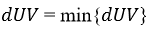
\includegraphics[scale=0.8] {gambarAHC/single.PNG}
    \label{fig:my_label}
\end{figure}

Keterangan : 
\par\textit{dUV} : adalah jarak antara data U dan V dari masing-masing cluster U dan V. 
\vspace{5cm}

\subsubsection{\textit{Average  Linkage}} 
\paragraph{}
\par \textit{Average  Linkage(AVERAGE)} menentukan kedekatan diantara dua kelompok dari jarak rata-rata antar dua data dari cluster yang berbeda. 
Formulasi untuk average linkage adalah : 
\begin{figure} [htbp]
    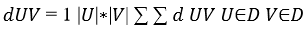
\includegraphics[scale=0.8] {gambarAHC/Average.PNG}
    \label{fig:my_label}
\end{figure}

Keterangan : 
\par U dan V adalah jumlah data yang ada dalam cluster U dan V. 
\vspace{1cm}

\subsubsection{\textit{Complete linkage}} 
\paragraph{}
\textit{Complete linkage(MAX)} menentukan kedekatan diantara dua kelompok dari jarak terjauh (terbesar) antara dua data dari cluster yang berbeda. Formulasi untuk complete linkage adalah : 

\par Formulasi untuk \textit{Single Linkage (MIN)} adalah :
\begin{figure} [htbp]
    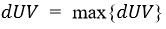
\includegraphics[scale=0.8] {gambarAHC/Complete.PNG}
    \label{fig:my_label}
\end{figure}

Keterangan : 
\par\textit{dUV} : adalah jarak antara data U dan V dari masing-masing cluster U 
dan V. 

\subsection{Implementasi \textit{Hierarchical Clustering}}
\subsubsection{implementasi \textit{Hierarchical Clustering} pada Data Musik}

\paragraph{}\textbf{Extraksi File Musik Dengan Feature Extraction Menggunakan Library Pyaudioanalysis}

\paragraph{}\hspace{0.5cm}PyAudioAnalysis dapat digunakan untuk mengekstrak fitur audio, melatih dan menerapkan pengklasifikasian audio, mensegmentasikan stream audio dan memvisualisasikan hubungan konten. Library  ini ditulis dengan Python, yang merupakan bahasa pemrograman tingkat tinggi yang telah menarik banyak peminat, terutama dalam komunitas akademis dan ilmiah selama beberapa tahun terakhir.\citep*{giannakopoulos2015pyaudioanalysis}  



Untuk dapat menggunakan fitur ekstraksi pada library  pyAudioAnalysis diharuskan melakukan tahap-tahap berikut ini: 
\begin{enumerate}
    \item Melakukan instalasi python
    \item Melakukan clone pada library  pyAudioAnalysis, sebelum perintah git clone dijalankan, terlebih dahulu masuk kedalam direktori yang diinginkan untuk menyimpanan Library  pyAudioAnalysis,  seperti “cd ujicoba”.
    \item inputkan perintah dibawah pada terminal untuk melakukan clone library   “git clone https://github.com/tyiannak/pyAudioAnalysis.git”.
\end{enumerate}
\begin{figure} [htbp]
    \centering
    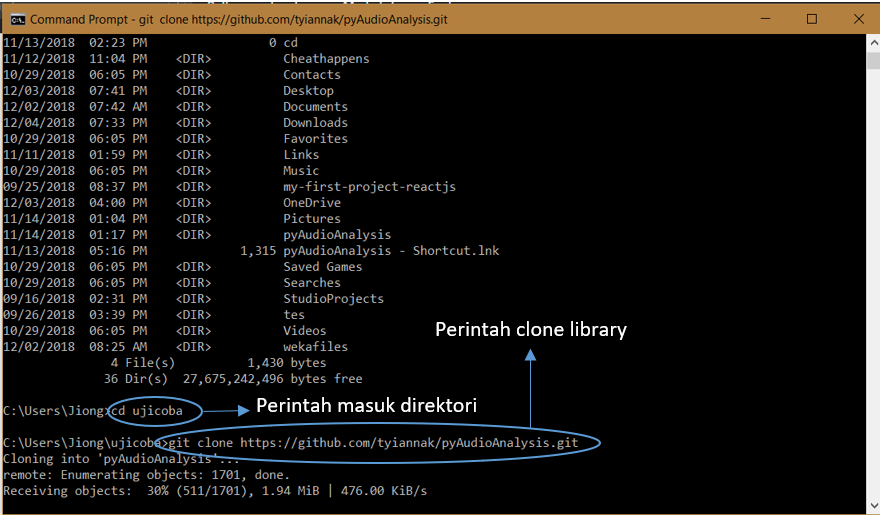
\includegraphics[scale=0.3] {gambarAHC/image009.png}
    \caption{\textit{ Clone library}}
\end{figure}



\paragraph{}\textbf{Install Dependencies Yang Digunakan Oleh Library  pyaudioanalysis }
\begin{enumerate}
    \item  NUMPY  : pip install numpy
    \par\hspace{1cm} Pada terminal terlihat dependencies NUMPY sudah terinstall dan file installan berada pada direktori c:\programdata\anaconda3\lib\sitepackages (1.15.1). Numpy adalah pustaka fundamental untuk perhitungan numerik menggunakan Python. Ini terutama digunakan untuk array,  representasi matriks dan penanganan, beserta dengan satu set fungsi array dasar masing-masing.
    
    \begin{figure} [htbp]
    \centering
    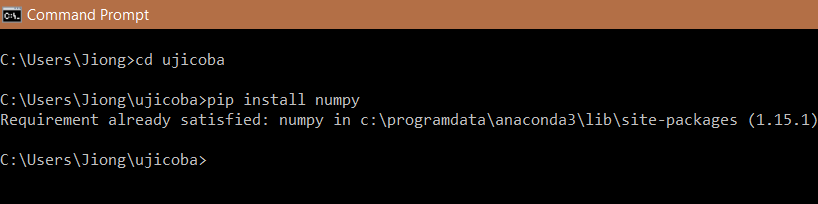
\includegraphics[scale=0.5] {gambarAHC/image011.png}
    \caption{\textit{ Install Dependencies NUMPY }}
    \end{figure}
  
    \vspace{5cm}
    \item MATPLOTLIB  : pip install matplotlib
    \par\hspace{1cm}Pada terminal terlihat dependencies MATPLOTLIB sudah terinstall dan file installan berada pada direktori c:\programdata\anaconda3\lib\sitepackages (2.2.3). Matplotlib menawarkan fungsionalitas penggambaran 2D, mirip dengan MATLAB
    
    \begin{figure} [htbp]
    \centering
    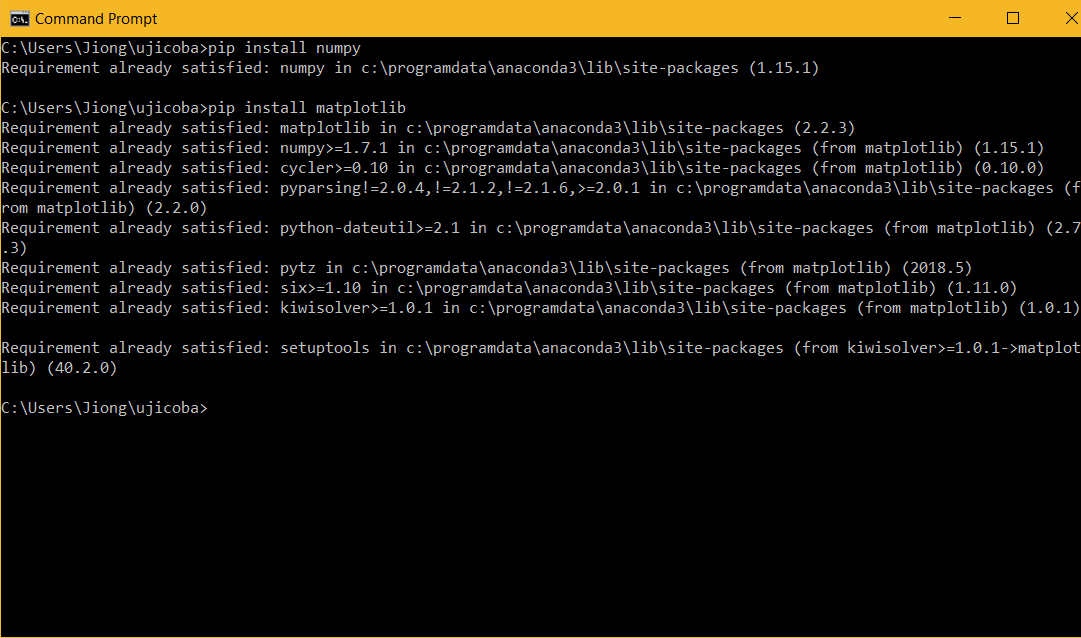
\includegraphics[scale=0.4] {gambarAHC/image013.png}
    \caption{\textit{ Install Dependencies MATPLOTLIB  }}
    \end{figure}
  
    
    \item SCIPY  : pip install scipy
    \par\hspace{1cm} Pada terminal terlihat dependencies SCIPY sudah terinstall dan file installan berada pada direktori c:\programdata\anaconda3\lib\sitepackages (1.1.0). SciPy adalah inti dari ekosistem berbasis SciPy Python yang menyediakan komputasi numerik yang dioptimalkan dan rutinitas ilmiah. pyAudioAnalysis menggunakan SciPy untuk prosedur pemrosesan sinyal dasar (misalnya konvolusi), perhitungan linear, perhitungan FFT dan file GELOMBANG IO. 
 
    \begin{figure} [htbp]
    \centering
    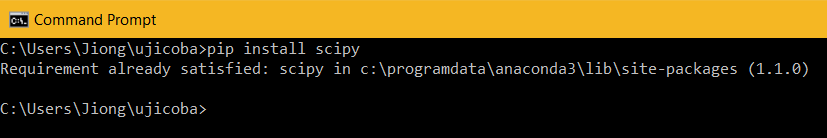
\includegraphics[scale=0.5] {gambarAHC/image015.png}
    \caption{\textit{ Install Dependencies SCIPY   }}
    \end{figure}
    
    \item SKLEARN   : pip install sklearn 
    \par\hspace{1cm} Pada terminal terlihat dependencies SKLEARN sudah terinstall dan file installan berada pada direktori c:\programdata\anaconda3\lib\sitepackages (0.0). SKLEARN adalah library  machine learning untuk bahasa pemrograman Python. Library  ini memiliki fitur seperti classification, regression dan algoritma clustering termasuk support vector machines, random forests , gradient boosting , k -means and DBSCAN, dan SKLEARN  dirancang untuk beroperasi dengan library  numerik dan ilmiah Python NumPy dan SciPy. 
 
    \begin{figure} [htbp]
    \centering
    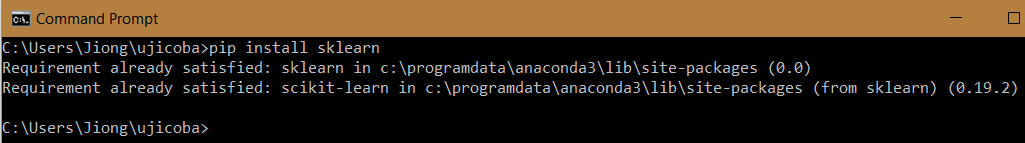
\includegraphics[scale=0.4] {gambarAHC/image017.png}
    \caption{\textit{ Install Dependencies SKLEARN   }}
    \end{figure}
    
     
    \item HMMLEARN    : pip install hmmlearn  
    \par\hspace{1cm} Pada terminal terlihat dependencies HMMLEARN sudah terinstall dan file installan berada pada direktori c:\programdata\anaconda3\lib\sitepackages (0.2.1). Library  HMMLEARN adalah algoritma dan model sederhana untuk mempelajari HMM ( Hidden Markov Models ) dengan Python, Dibangun dalam library  scikit-learn, NumPy, SciPy, dan matplotlib. Library  HMMLEARN merupakan library  Open source dan dapat digunakan secara komersial.
 
    \begin{figure} [htbp]
    \centering
    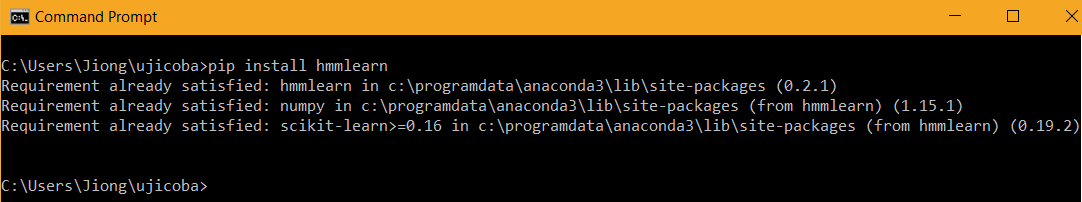
\includegraphics[scale=0.4] {gambarAHC/image019.png}
    \caption{\textit{ Install Dependencies hmmlearn    }}
    \end{figure}
   
      
    \item Simplejson     : pip install Simplejson   
    \par\hspace{1cm} Pada terminal terlihat dependencies Simplejson sudah terinstall dan file installan berada pada direktori c:\programdata\anaconda3\lib\sitepackages (3.16.0). Library  Simplejson memaparkan API dari library  marshal dan modul pickle . Ini adalah versi library  json dipelihara secara eksternal yang terdapat dalam Python 2.6, tetapi mempertahankan kompatibilitas dengan Python 2.5 dan memiliki keunggulan kinerja yang signifikan, bahkan tanpa menggunakan ekstensi C opsional untuk percepatan. simplejson juga didukung pada Python 3.3+. 
 
    \begin{figure} [htbp]
    \centering
    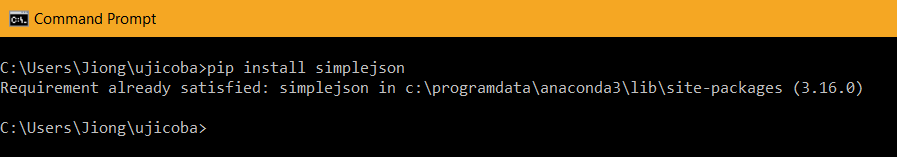
\includegraphics[scale=0.5] {gambarAHC/image021.png}
    \caption{\textit{ Install Dependencies Simplejson    }}
    \end{figure}
     

      \item eyeD3      : pip install eyeD3    
    \par\hspace{1cm} Pada terminal terlihat dependencies eyeD3 sudah terinstall dan file installan berada pada direktori c:\programdata\anaconda3\lib\sitepackages (0.8.7). eyeD3 adalah tools dari Python untuk bekerja dengan file audio, khususnya file MP3 yang berisi metadata ID3 (yaitu info lagu), misalnya untuk mengatur beberapa informasi lagu dalam file mp3. Library  ini menyediakan command-line tool (eyeD3) dan library  Python ( import eyed3 ) yang dapat digunakan untuk menulis aplikasi anda sendiri yang dapat dipanggil dari command-line tool. 
 
  
 
    \begin{figure} [htbp]
    \centering
    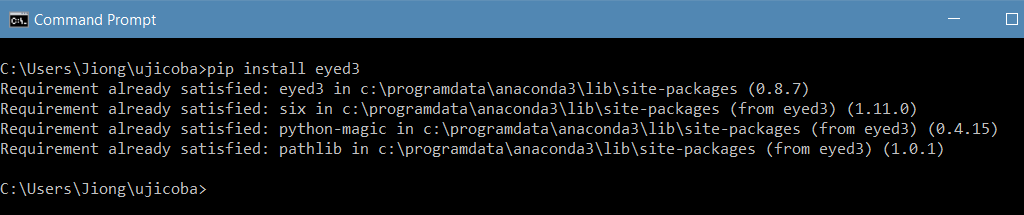
\includegraphics[scale=0.5] {gambarAHC/image023.png}
    \caption{\textit{ Install Dependencies eyeD3     }}
    \end{figure}
    
          \item pydub       : pip install pydub     
    \par\hspace{1cm} Pada terminal terlihat dependencies pydub sudah terinstall dan file installan berada pada direktori c:\programdata\anaconda3\lib\sitepackages (0.23.0). 
 \begin{figure} [htbp]
    \centering
    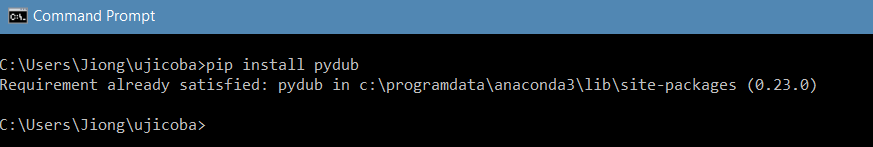
\includegraphics[scale=0.5] {gambarAHC/image025.png}
    \caption{\textit{ Install Dependencies pydub}}
    \end{figure}
\end{enumerate}


  \paragraph{}\textbf{Mengubah Format File Musik Dari Mp3 Mejadi Wav }
    \paragraph{}\hspace{1cm}Library  sudah dapat digunakan, sebelum menjalankan feature extraction file musik harus di rubah kedalam format WAV, dengan perintah berikut: “python audioAnalysis.py dirMp3toWav -i datamusik/ -r 16000 -c 1” Perintah diatas mengubah data musik yang berada pada direktori datamusik    dari format mp3 menjadi WAV. \begin{figure} [htbp]
    \centering
    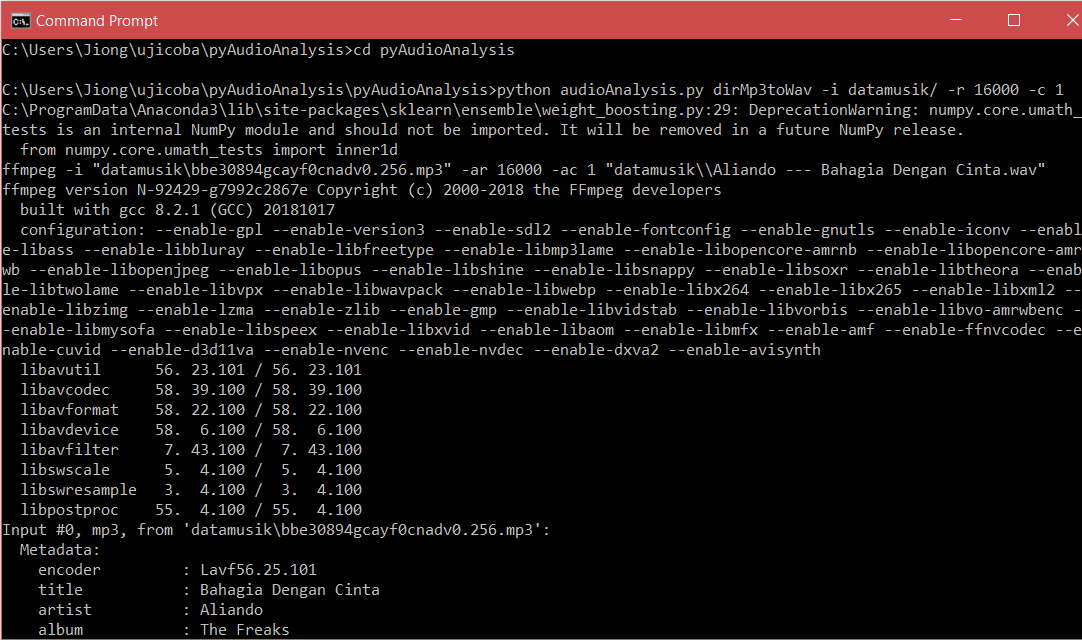
\includegraphics[scale=0.35] {gambarAHC/image027.png}
    \caption{\textit{ convert mp3 to WAV}}
    \end{figure}
    \vspace{5cm}

    \paragraph{}\hspace{1cm}Pada gambar dibawah terlihat semua file musik pada direktori datamusik sudah diubah menjadi file yang memiliki format .WAV  dari yang awalnya berformat mp3. 
    \begin{figure} [htbp]
    \centering
    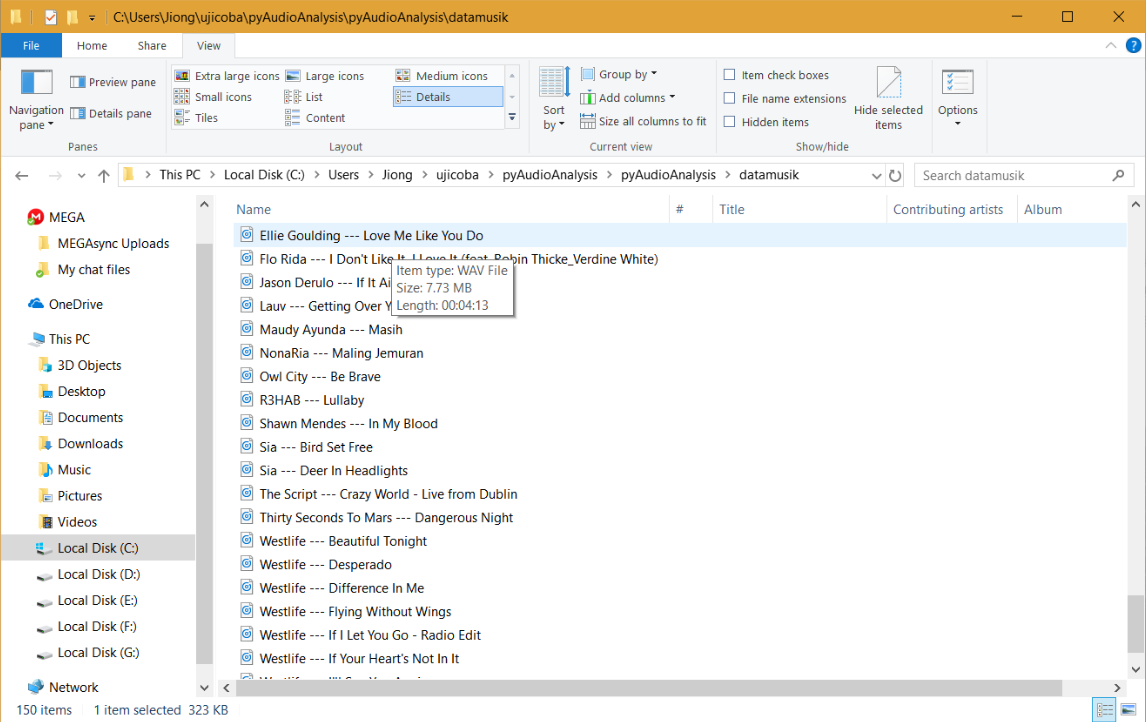
\includegraphics[scale=0.4] {gambarAHC/realimage029.PNG}
    \caption{\textit{ Hasil convert mp3 to WAV }}
    \end{figure}

\paragraph{}\textbf{Menjalankan Ekstraksi Musik Menggunakan Feature Extraction}
    \paragraph{}\hspace{1cm}Menjalankan fungsi feature extraction pada library  pyAudioAnalysis dengan  perintah : “python audioAnalysis.py  featureExtractionDir -i datamusik / -mw 1.0 -ms 1.0 -sw 0.050 -ss 0.050”.  Perintah ini akan mengekstrak semua file musik yang memiliki format .WAV pada direktori datamusik yang memiliki output CSV.  \begin{figure} [htbp]
    \centering
    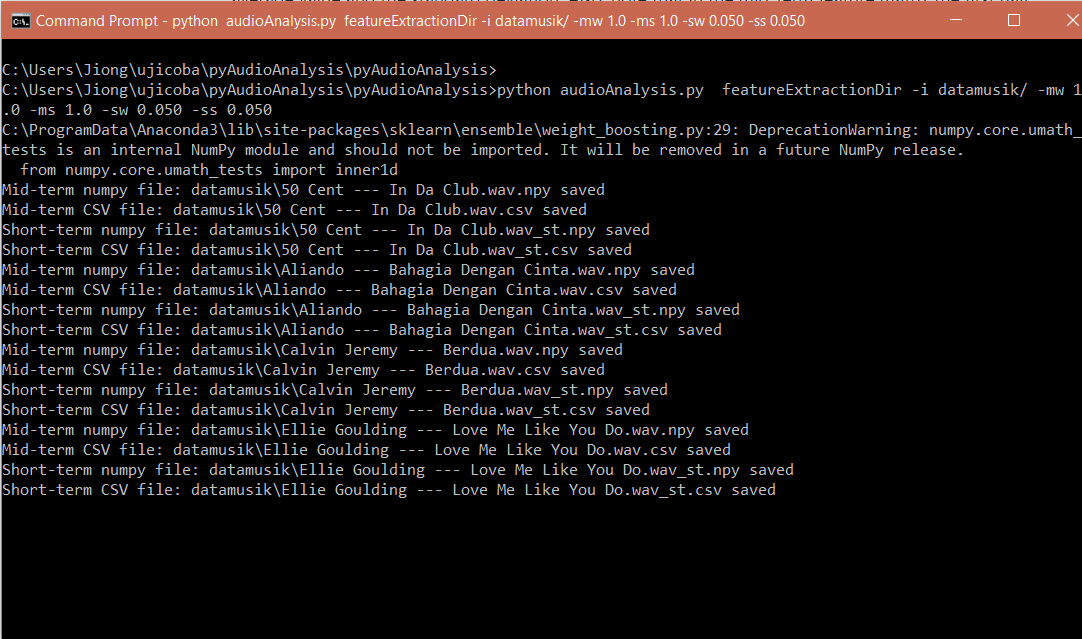
\includegraphics[scale=0.4] {gambarAHC/image031.png}
    \caption{\textit{fungsi feature extraction }}
    \end{figure}
    
    Pada gambar dibawah terlihat semua file musik pada direktori data musik yang memiliki format .WAV  sudah diekstraksi dan hasil ekstraksi setiap lagu akan menghasilkan  file csv. Kemudian data tersebut di processing dengan menggabungkan semua data kedalam 1 file csv. 
     \begin{figure} [htbp]
    \centering
    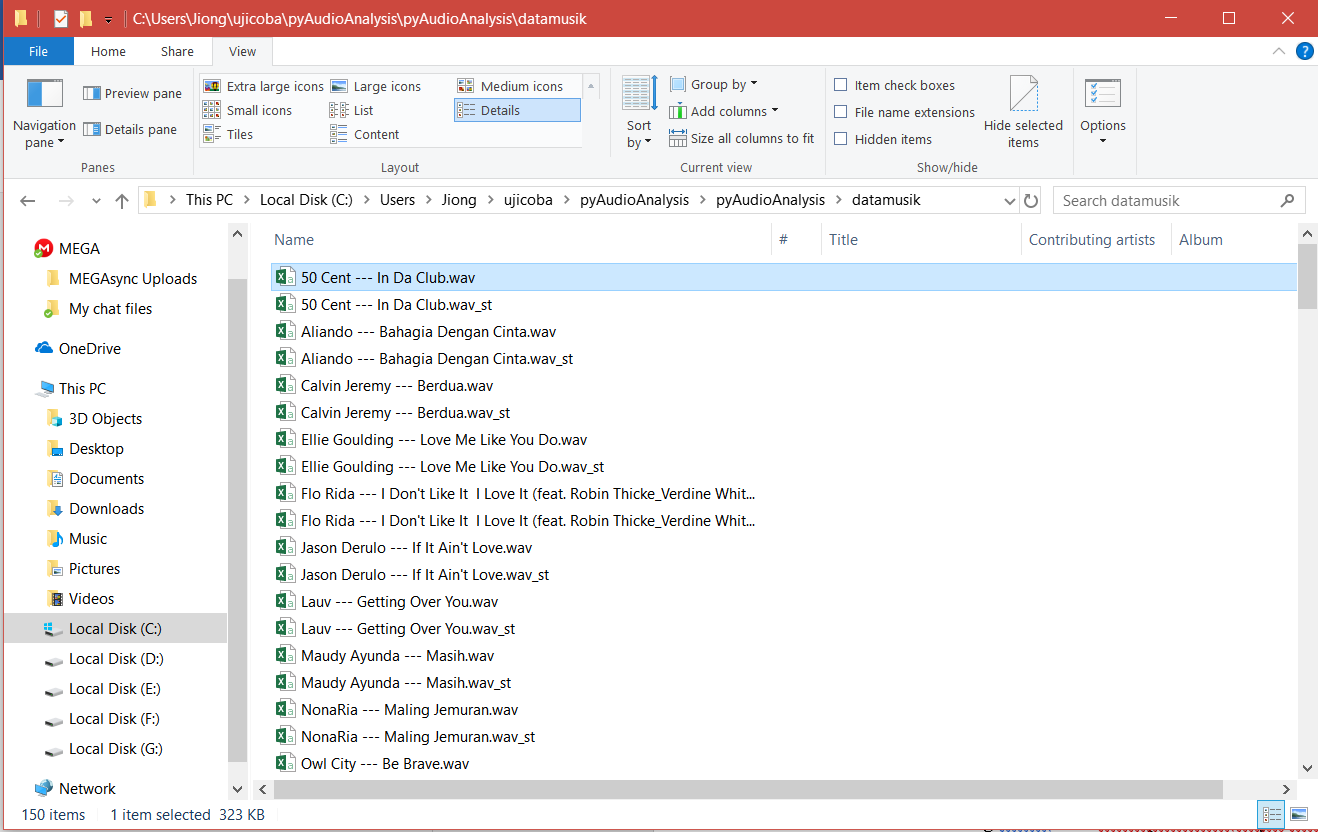
\includegraphics[scale=0.35] {gambarAHC/image033.png}
    \caption{\textit{Output fungsi feature extraction}}
    \end{figure}
  
\paragraph{}\textbf{Penerapan Algoritma Agglomerative Hierachical Pada Content Musik} 

% Please add the following required packages to your document preamble:
% \usepackage{graphicx}
% \usepackage[normalem]{ulem}
% \useunder{\uline}{\ul}{}
\begin{table}[htbp]
\captionsetup{singlelinecheck=off}
\caption{Nilai atribut tiap musik}
\label{test}
\resizebox{\textwidth}{!}{%
\begin{tabular}{|l|l|l|l|l|l|l|l|l|l|l|l|}
\hline
Judul & \begin{tabular}[c]{@{}l@{}}Zero Crossing \\ Rate\end{tabular} & Energy & \begin{tabular}[c]{@{}l@{}}Entropy \\ of Energy\end{tabular} & \begin{tabular}[c]{@{}l@{}}Spectral \\ Centroid\end{tabular} & \begin{tabular}[c]{@{}l@{}}Spectral \\ Spread\end{tabular} & \begin{tabular}[c]{@{}l@{}}Spectral \\ Entropy\end{tabular} & \begin{tabular}[c]{@{}l@{}}Spectral\\ Flux\end{tabular} & \begin{tabular}[c]{@{}l@{}}Spectral \\ Rolloff\end{tabular} & MFCCs & \begin{tabular}[c]{@{}l@{}}Chroma \\ Vector\end{tabular} & \begin{tabular}[c]{@{}l@{}}Chroma \\ Deviation\end{tabular} \\ \hline
1 & 0.11 & 0.05 & 3.14 & 0.20 & 0.22 & 0.96 & 0.01 & 0.16 & -1.69 & 0.02 & 0.03 \\ \hline
2 & 0.12 & 0.07 & 3.19 & 0.23 & 0.23 & 1.10 & 0.01 & 0.21 & -1.67 & 0.02 & 0.03 \\ \hline
3 & 0.11 & 0.09 & 3.17 & 0.24 & 0.25 & 0.93 & 0.01 & 0.18 & -1.67 & 0.02 & 0.04 \\ \hline
4 & 0.07 & 0.02 & 3.17 & 0.15 & 0.20 & 0.42 & 0.01 & 0.09 & -1.80 & 0.02 & 0.03 \\ \hline
5 & 0.10 & 0.09 & 3.13 & 0.23 & 0.25 & 0.81 & 0.01 & 0.16 & -1.57 & 0.02 & 0.04 \\ \hline
6 & 0.07 & 0.04 & 3.17 & 0.17 & 0.21 & 0.48 & 0.01 & 0.10 & -1.67 & 0.02 & 0.04 \\ \hline
7 & 0.09 & 0.05 & 3.17 & 0.21 & 0.23 & 0.70 & 0.02 & 0.15 & -1.75 & 0.02 & 0.06 \\ \hline
8 & 0.10 & 0.05 & 3.16 & 0.20 & 0.21 & 0.88 & 0.01 & 0.16 & -1.82 & 0.02 & 0.04 \\ \hline
9 & 0.10 & 0.07 & 3.16 & 0.23 & 0.24 & 0.91 & 0.01 & 0.17 & -1.58 & 0.02 & 0.05 \\ \hline
10 & 0.14 & 0.06 & 3.22 & 0.25 & 0.24 & 1.28 & 0.01 & 0.23 & -1.64 & 0.02 & 0.03 \\ \hline
\end{tabular}%
}
\end{table}
\vspace{5cm}

% Please add the following required packages to your document preamble:
% \usepackage{graphicx}
\begin{table}[htbp]
\captionsetup{singlelinecheck=off}
\caption{Penamaan musik}
\label{tab:my-table}
\resizebox{0.8\textwidth}{!}{%
\begin{tabular}{|l|l|}
\hline
\textbf{Inisial} & \textbf{Judul} \\ \hline
1 & Aliando --- Jatuh Cinta Tak Ada Logika \\ \hline
2 & Anne-Marie --- Ciao Adios \\ \hline
3 & bruno mars- just the way you are \\ \hline
4 & Hanin Dhiya --- Darling – Acoustic \\ \hline
5 & Jason Derulo --- Colors \\ \hline
6 & Jason Mraz --- Bella Luna \\ \hline
7 & Jessie J --- I Got You (I Feel Good) \\ \hline
8 & Julia Michaels --- Issues \\ \hline
9 & Calum Scott --- Give Me Something \\ \hline
10 & linkin park- burn it down \\ \hline
\end{tabular}%
}
\end{table}

% Please add the following required packages to your document preamble:
% \usepackage{graphicx}
\begin{table}[htbp]
\captionsetup{singlelinecheck=off}
\caption{Kriteria Kluster}
\label{tab:my-table}
\resizebox{0.8\textwidth}{!}{%
\begin{tabular}{|l|l|}
\hline
Kluster & Kriteria \\ \hline
K1 & Contenment (menenangkan, relaksasi, damai) \\ \hline
K2 & Exuberance (riuh, bersemangat, bergembira) \\ \hline
K3 & Depression (sedih, murung, depresi, duka) \\ \hline
K4 & Anxious (amarah, kacau, konflik) \\ \hline
\end{tabular}%
}
\end{table}

\vspace{5cm}
\begin{enumerate}
    \item  Dari data ekstraksi musik pada Tabel \ref{test} akan dihitung  matrik jarak antar data menggunakan matrik Euclidian Distance, dengan rumus :
    \begin{figure} [htbp]
    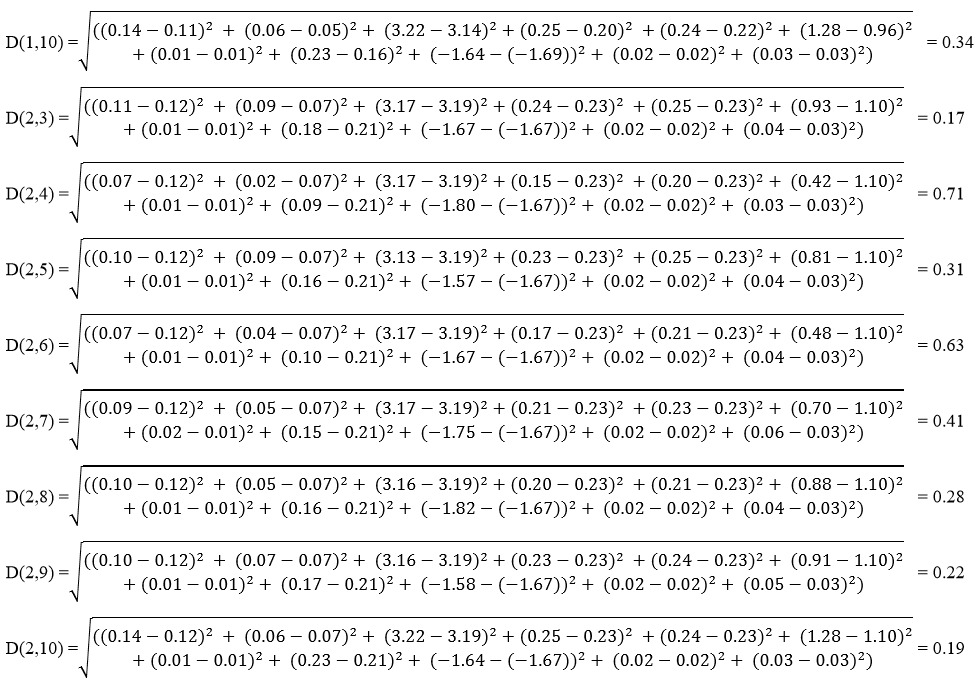
\includegraphics[scale=0.55] {gambarAHC/AHC1.PNG}
    \end{figure}
    
    \begin{figure} [htbp]
    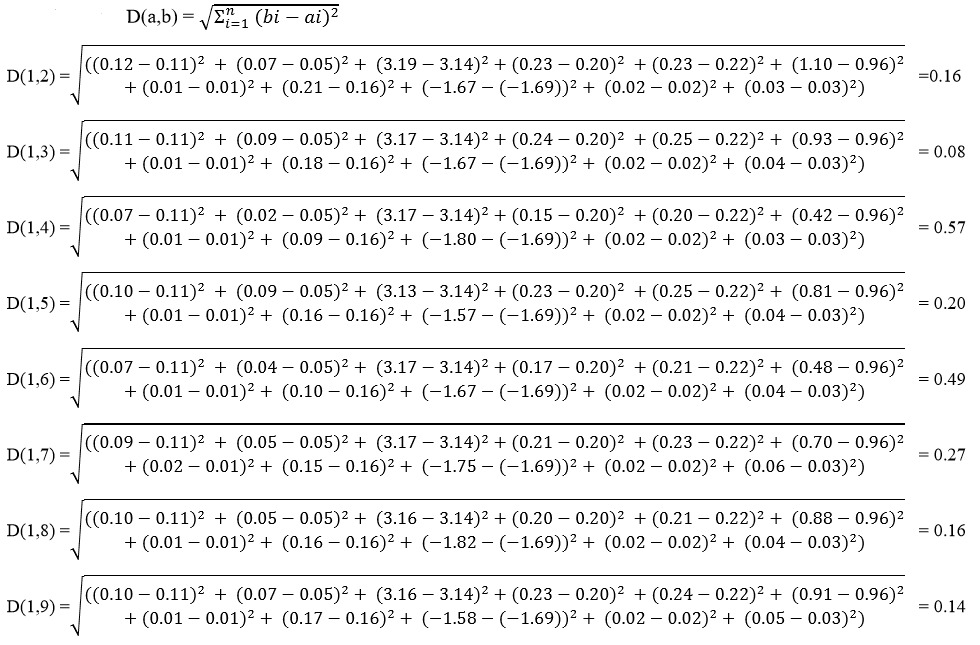
\includegraphics[scale=0.55] {gambarAHC/AHC2.PNG}
    \end{figure}
    \vspace{4cm}
    
    \begin{figure} [htbp]
    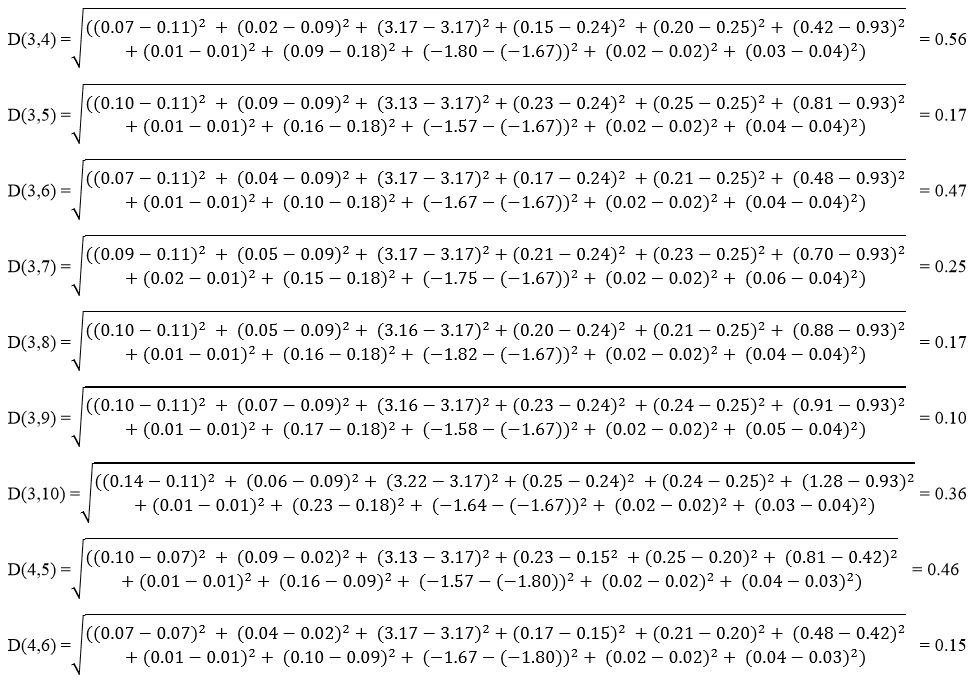
\includegraphics[scale=0.53] {gambarAHC/AHC3.PNG}
    \end{figure}
       
    
    \begin{figure} [htbp]
    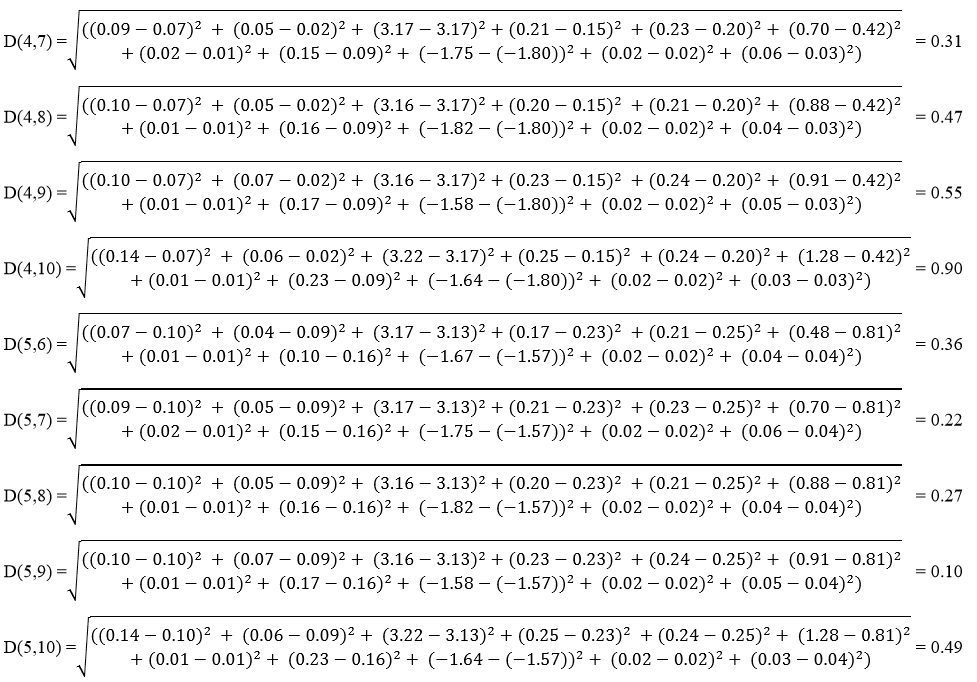
\includegraphics[scale=0.53] {gambarAHC/AHC4.PNG}
    \end{figure}
       \vspace{5cm}

    
    \begin{figure} [htbp]
    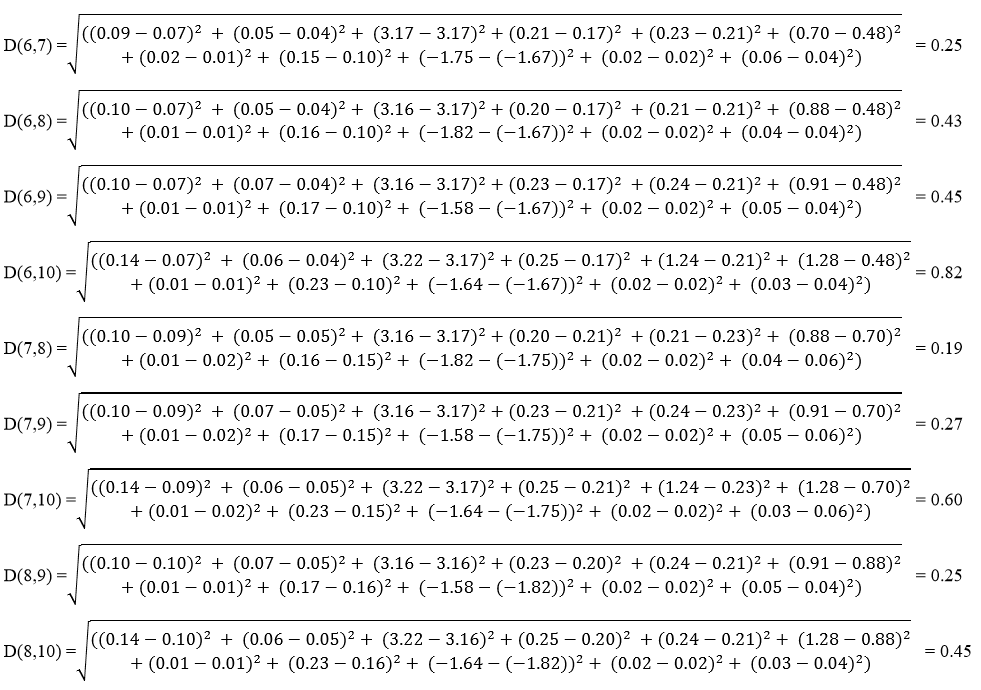
\includegraphics[scale=0.52] {gambarAHC/AHC5.PNG}
    \end{figure}
   
    \begin{figure} [htbp]
    \includegraphics[scale=0.7] {gambarAHC/66.PNG}
    \end{figure}
       \vspace{6cm}
    
% Please add the following required packages to your document preamble:
% \usepackage{graphicx}
\begin{table}[htbp]
\captionsetup{singlelinecheck=off}
\caption{Matrik Jarak, dengan Euclidian Distance}
\label{tab:my-table}
\resizebox{0.7\textwidth}{!}{%
\begin{tabular}{|l|l|l|l|l|l|l|l|l|l|l|}
\hline
 & 1 & 2 & 3 & 4 & 5 & 6 & 7 & 8 & 9 & 10 \\ \hline
1 &  & 0.16 & 0.08 & 0.57 & 0.20 & 0.49 & 0.27 & 0.16 & 0.14 & 0.34 \\ \hline
2 & 0.16 &  & 0.17 & 0.71 & 0.31 & 0.63 & 0.41 & 0.28 & 0.22 & 0.19 \\ \hline
3 & 0.08 & 0.17 &  & 0.56 & 0.17 & 0.47 & 0.25 & 0.17 & 0.10 & 0.36 \\ \hline
4 & 0.57 & 0.71 & 0.56 &  & 0.48 & 0.15 & 0.31 & 0.47 & 0.55 & 0.90 \\ \hline
5 & 0.20 & 0.31 & 0.17 & 0.48 &  & 0.36 & 0.22 & 0.27 & 0.10 & 0.49 \\ \hline
6 & 0.49 & 0.63 & 0.47 & 0.15 & 0.36 &  & 0.25 & 0.43 & 0.45 & 0.82 \\ \hline
7 & 0.27 & 0.41 & 0.25 & 0.31 & 0.22 & 0.25 &  & 0.19 & 0.27 & 0.60 \\ \hline
8 & 0.16 & 0.28 & 0.17 & 0.47 & 0.27 & 0.43 & 0.19 &  & 0.25 & 0.45 \\ \hline
9 & 0.14 & 0.22 & 0.10 & 0.55 & 0.10 & 0.45 & 0.27 & 0.25 &  & 0.39 \\ \hline
10 & 0.34 & 0.19 & 0.36 & 0.90 & 0.49 & 0.82 & 0.60 & 0.45 & 0.39 &  \\ \hline
\end{tabular}%
}
\end{table}

\item Dengan metode complete linkage, selanjutnya dipilih dua jarak cluster yang paling terkecil =MIN(B2:K11) = d13 = 0.08
Perhitungan awal cluster (13) tetap digunakan dikarenakan cluster (13) memiliki jarak paling dekat. Maka dipilih cluster 1 dan 3, sehingga cluster 1 dan 3 digabungkan. Selanjutnya, akan dihitung jarak-jarak antara cluster (13) dengan cluster 2,4,5,6,7,8,9 dan 10.

D(13)2 = MAX(0.16, 0.17) = 0.17

D(13)4 = MAX(0.57, 0.56) = 0.57

D(13)5 = MAX(0.20, 0.17) = 0.17

D(13)6 = MAX(0.49, 0.47) = 0.49

D(13)7 = MAX(0.27, 0.25) = 0.57

D(13)8 = MAX(0.16, 0.17) = 0.17

D(13)9 = MAX(0.14, 0.10) = 0.14

D(13)10 = MAX(0.34, 0.36) = 0.36

% Please add the following required packages to your document preamble:
% \usepackage{graphicx}
\begin{table}[htbp]
\captionsetup{singlelinecheck=off}
\caption{Matrik Jarak, d(1,3)}
\label{tab:my-table}
\resizebox{0.6\textwidth}{!}{%
\begin{tabular}{|l|l|l|l|l|l|l|l|l|l|}
\hline
\textbf{} & \textbf{1,3} & \textbf{2} & \textbf{4} & \textbf{5} & \textbf{6} & \textbf{7} & \textbf{8} & \textbf{9} & \textbf{10} \\ \hline
\textbf{1,3} &  & 0.17 & 0.57 & 0.20 & 0.49 & 0.27 & 0.17 & 0.14 & 0.36 \\ \hline
\textbf{2} &  &  & 0.71 & 0.31 & 0.63 & 0.41 & 0.28 & 0.22 & 0.19 \\ \hline
\textbf{4} &  &  &  & 0.48 & 0.15 & 0.31 & 0.47 & 0.55 & 0.90 \\ \hline
\textbf{5} &  &  &  &  & 0.36 & 0.22 & 0.27 & \textbf{0.10} & 0.49 \\ \hline
\textbf{6} &  &  &  &  &  & 0.25 & 0.43 & 0.45 & 0.82 \\ \hline
\textbf{7} &  &  &  &  &  &  & 0.19 & 0.27 & 0.60 \\ \hline
\textbf{8} &  &  &  &  &  &  &  & 0.25 & 0.45 \\ \hline
\textbf{9} &  &  &  &  &  &  &  &  & 0.39 \\ \hline
\textbf{10} &  &  &  &  &  &  &  &  &  \\ \hline
\end{tabular}%
}
\end{table}

Selanjutnya dipilih kembali jarak dua cluster terkecil. min(\textbf{dUV} \textit{d}(5,9) = 0.10 dan hitung kembali jarak-jarak antara cluster (5,9) dengan cluster yang tersisa 1.3,2,4,6,7,8 dan 10.

D(5,9)13 = MAX(0.20, 0.14, 0.17, 0.10) = 0.20

D(5,9)2  = MAX(0.31, 0.22) = 0.31

D(5,9)4 = MAX(0.48, 0.55) = 0.55

D(5,9)6 = MAX(0.36, 0.45) = 0.45

D(5,9)7 = MAX(0.22, 0.22) = 0.27

D(5,9)8 = MAX(0.27, 0.25) = 0.27

D(5,9)10 = MAX(0.49, 0.36) = 0.49


% Please add the following required packages to your document preamble:
% \usepackage{graphicx}
\begin{table}[htbp]
\captionsetup{singlelinecheck=off}
\caption{Matrik Jarak, d(5,9)}
\label{tab:my-table}
\resizebox{0.6\textwidth}{!}{%
\begin{tabular}{|l|l|l|l|l|l|l|l|l|}
\hline
\textbf{} & \textbf{1,3} & \textbf{2} & \textbf{4} & \textbf{5,9} & \textbf{6} & \textbf{7} & \textbf{8} & \textbf{10} \\ \hline
\textbf{1,3} &  & 0.17 & 0.57 & 0.20 & 0.49 & 0.27 & 0.17 & 0.36 \\ \hline
\textbf{2} &  &  & 0.71 & 0.31 & 0.63 & 0.41 & 0.28 & 0.19 \\ \hline
\textbf{4} &  &  &  & 0.55 & \textbf{0.15} & 0.31 & 0.47 & 0.90 \\ \hline
\textbf{5,9} &  &  &  &  & 0.45 & 0.27 & 0.27 & 0.49 \\ \hline
\textbf{6} &  &  &  &  &  & 0.25 & 0.43 & 0.82 \\ \hline
\textbf{7} &  &  &  &  &  &  & 0.19 & 0.60 \\ \hline
\textbf{8} &  &  &  &  &  &  &  & 0.45 \\ \hline
\textbf{10} &  &  &  &  &  &  &  &  \\ \hline
\end{tabular}%
}
\end{table}

Selanjutnya dipilih kembali jarak dua cluster terkecil. min\textit{(dUV)}=4,6) = 0.15 dan hitung kembali jarak-jarak antara cluster (4,6)  dengan cluster yang tersisa 1.3,2,5.9,7,8 dan 10.

D(4,6)13=MAX (0.57,0.56,0.49,0.47)=0.57

D(4,6)2=MAX (0.71,0.63)=0.71

D(4,6)5,9=MAX (0.48,0.55,0.36,0.45)=0.55

D(4,6)7=MAX (0.31,0.25)=0.31

D(4,6)8=MAX (0.47,0.43)=0.47

D(4,6)10=MAX (0.90,0.82)=0.90

% Please add the following required packages to your document preamble:
% \usepackage{graphicx}
\begin{table}[htbp]
\captionsetup{singlelinecheck=off}
\caption{Matrik Jarak, d(4,6)}
\label{tab:my-table}
\resizebox{0.6\textwidth}{!}{%
\begin{tabular}{|l|l|l|l|l|l|l|l|}
\hline
\textbf{} & \textbf{1,3} & \textbf{2} & \textbf{4,6} & \textbf{5,9} & \textbf{7} & \textbf{8} & \textbf{10} \\ \hline
\textbf{1,3} &  & \textbf{0.17} & 0.57 & 0.20 & 0.27 & 0.17 & 0.36 \\ \hline
\textbf{2} &  &  & 0.71 & 0.31 & 0.41 & 0.28 & 0.19 \\ \hline
\textbf{4,6} &  &  &  & 0.55 & 0.31 & 0.47 & 0.90 \\ \hline
\textbf{5,9} &  &  &  &  & 0.27 & 0.27 & 0.49 \\ \hline
\textbf{7} &  &  &  &  &  & 0.19 & 0.60 \\ \hline
\textbf{8} &  &  &  &  &  &  & 0.45 \\ \hline
\textbf{10} &  &  &  &  &  &  &  \\ \hline
\end{tabular}%
}
\end{table}

Selanjutnya dipilih kembali jarak dua cluster terkecil. min\textit{(dUV)}= d(1,3,2) = 0.17 dan hitung kembali jarak-jarak antara cluster (1,3,2)  dengan cluster yang tersisa 4.6,5.9,7,8 dan 10.

D(1,3,2)4,6 = MAX(0.57,0.56,0.71,0.49,0.47,0.43)=0.71

D(1,3,2)5,9 = MAX(0.20,0.17,0.31,0.14,0.10,0.22)=0.31

D(1,3,2)7 = MAX(0.27,0.25,0.41)=0.41

D(1,3,2)8 = MAX(0.16,0.17,0.28)=0.28

D(1,3,2)10 = MAX(0.34,0.36,0.19)=0.36

% Please add the following required packages to your document preamble:
% \usepackage{graphicx}
\begin{table}[htbp]
\captionsetup{singlelinecheck=off}
\caption{ Matrik Jarak, d(1,3,2}
\label{tab:my-table}
\resizebox{0.4\textwidth}{!}{%
\begin{tabular}{|l|l|l|l|l|l|l|}
\hline
\textbf{} & \textbf{1,3,2} & \textbf{4,6} & \textbf{5,9} & \textbf{7} & \textbf{8} & \textbf{10} \\ \hline
\textbf{1,3,2} &  & 0.71 & 0.31 & 0.41 & 0.28 & 0.36 \\ \hline
\textbf{4,6} &  &  & 0.55 & 0.31 & 0.27 & 0.90 \\ \hline
\textbf{5,9} &  &  &  & 0.27 & 0.27 & 0.49 \\ \hline
\textbf{7} &  &  &  &  & \textbf{0.19} & 0.60 \\ \hline
\textbf{8} &  &  &  &  &  & 0.45 \\ \hline
\textbf{10} &  &  &  &  &  &  \\ \hline
\end{tabular}%
}
\end{table}

Selanjutnya dipilih kembali jarak dua cluster terkecil. min\textit{(dUV)} \textit{d}(7,8) = 0.19 dan hitung kembali jarak-jarak antara cluster (7,8)  dengan cluster yang tersisa 1.3.2,4.6,5.9, dan 10. 

D(7,8)1,3,2 = MAX(0.27,0.25,0.41,0.16,0.17,0.28)=0.41 
 
D(7,8)4,6 = MAX(0.31,0.25,0.47,0.43)=0.47 

D(7,8)5,9 = MAX(0.22,0.27,0.27,0.25)=0.27 

D(7,8)10 = MAX(0.60,0.45)=0.60 
 
% Please add the following required packages to your document preamble:
% \usepackage{graphicx}
\begin{table}[htbp]
\captionsetup{singlelinecheck=off}
\caption{ Matrik Jarak, d(7,8) }
\label{tab:my-table}
\resizebox{0.4\textwidth}{!}{%
\begin{tabular}{|l|l|l|l|l|l|}
\hline
\textbf{} & \textbf{1,3,2} & \textbf{4,6} & \textbf{5,9} & \textbf{7,8} & \textbf{10} \\ \hline
\textbf{1,3,2} &  & 0.71 & 0.31 & 0.41 & 0.36 \\ \hline
\textbf{4,6} &  &  & 0.55 & 0.47 & 0.90 \\ \hline
\textbf{5,9} &  &  &  & \textbf{0.27} & 0.49 \\ \hline
\textbf{7,8} &  &  &  &  & 0.60 \\ \hline
\textbf{10} &  &  &  &  &  \\ \hline
\end{tabular}%
}
\end{table}

Selanjutnya dipilih kembali jarak dua cluster terkecil. min\textit{(dUV)} \textit{d}(5,9,7,8) = 0.27 dan hitung kembali jarak-jarak antara cluster (5,9,7,8)  dengan cluster yang tersisa 1.3.2,4.6 dan 10.

D(5,9,7,8)1,3,2 = MAX(0.20,0.17,0.31,0.14,0.10,0.22,0.27,0.25,0.41,0.16,0.17,\\0.28)=0.41

D(5,9,7,8)4,6 = MAX(0.48,0.36,0.55,0.45,0.31.0.25,0.47,0.43)=0.55

D(5,9,7,8)10 = MAX(0.49,0.39,0.60,0.45)=0.60

\vspace{5cm}
% Please add the following required packages to your document preamble:
% \usepackage{graphicx}
\begin{table}[htbp]
\captionsetup{singlelinecheck=off}
\caption{Matrik Jarak, d(5,9,7,8)}
\label{tab:my-table}
\resizebox{0.4\textwidth}{!}{%
\begin{tabular}{|l|l|l|l|l|}
\hline
\textbf{} & \textbf{1,3,2} & \textbf{4,6} & \textbf{5,9,7,8} & \textbf{10} \\ \hline
\textbf{1,3,2} &  & 0.71 & 0.41 & 0.36 \\ \hline
\textbf{4,6} &  &  & 0.55 & 0.90 \\ \hline
\textbf{5,9,7,8} &  &  &  & 0.60 \\ \hline
\textbf{10} &  &  &  &  \\ \hline
\end{tabular}%
}
\end{table}
\end{enumerate}

Hasil akhir dari perhitungan keseluruhan matriks sudah menghasilkan 4 kluster sesuai yang ditentukan sejak awal.

Kluster 1 : (1) Aliando --- Jatuh Cinta Tak Ada Logika, (3) bruno mars- just the             way you are, (2) Anne-Marie --- Ciao Adios

Kluster 2 : (4)Hanin Dhiya --- Darling - Acoustic, (6) Jason Mraz --- Bella Luna

Kluster 3 : (5) Jason Derulo --- Colors, (9) Calum Scott --- Give Me Something,              (7) Jessie J --- I Got You (I Feel Good), (8) Julia Michaels --- Issues

Kluster 4 : (10) linkin park- burn it down

\subsection{ Validasi Hasil Perhitungan Agglomerative Hierarchical Clustering menngunakan tools RapidMiner}
 \begin{figure} [htbp]
    \includegraphics[scale=0.28] {gambarAHC/7.PNG}
    \end{figure}
    \vspace{5cm}

\subsection{Soal Latihan}
\begin{enumerate}
    \item Ekstraklah 25 data musik menggunakan library python Pyaudioanalysis lalu implementasikan Metode \textit{Agglomerative Hierarchical clustering} dengan menggunakan teknik pendekatan : \textit{single linkage}, \textit{complete linkage} dan \textit{ average linkage}, banyak kluster berdasarkan 4 kriteria kluster pada contoh soal dan berikan alasan untuk setiap kluster mengapa musik tersebut tergabung pada kluster itu.
    \item Pada tabel dibawah terdapat data ukuran badan mahasiswa, kelompokanlah data tersebut menjadi 2 kelompok dengan menggunakan teknik pendekatan : \textit{single linkage}, \textit{complete linkage} dan \textit{ average linkage}. 
    % Please add the following required packages to your document preamble:
% \usepackage{graphicx}
\begin{table}[htbp]

\label{tab:my-table}
\resizebox{\textwidth}{!}{%
\begin{tabular}{|c|c|c|c|c|c|}
\hline
\multicolumn{1}{|l|}{\textbf{Nama}} & \multicolumn{1}{l|}{\textbf{Tinggi(cm)}} & \multicolumn{1}{l|}{\textbf{Berat(kg)}} & \multicolumn{1}{l|}{\textbf{\begin{tabular}[c]{@{}l@{}}Lingkar  \\ Tangan(cm)\end{tabular}}} & \multicolumn{1}{l|}{\textbf{\begin{tabular}[c]{@{}l@{}}Lingkar \\ Pinggang(cm)\end{tabular}}} & \multicolumn{1}{l|}{\textbf{\begin{tabular}[c]{@{}l@{}}Lingkar \\ Paha(cm)\end{tabular}}} \\ \hline
Brandon & 180 & 88 & 40 & 64 & 75 \\ \hline
Kent & 155 & 68 & 50 & 68 & 67 \\ \hline
Jess & 189 & 77 & 55 & 69 & 51 \\ \hline
Zxuan & 200 & 79 & 45 & 84 & 59 \\ \hline
Bruno & 178 & 65 & 35 & 70 & 88 \\ \hline
Lesley & 188 & 59 & 34 & 75 & 77 \\ \hline
Granger & 198 & 57 & 24 & 88 & 66 \\ \hline
Fanny & 145 & 68 & 28 & 94 & 51 \\ \hline
Lancelot & 154 & 99 & 51 & 58 & 48 \\ \hline
Rias Gremory & 165 & 91 & 26 & 64 & 77 \\ \hline
\end{tabular}%
}
\end{table}
\end{enumerate}




